\documentclass{article}

\usepackage{Sweave}
\begin{document}
\Sconcordance{concordance:plot_test.tex:plot_test.Rnw:%
1 8 1 1 0 51 1 1 2 1 0 7 1 3 0 1 2 3 1 1 2 1 0 1 1 3 0 1 2 2 1 1 -4 1 8 %
8 1}


\section*{plot test}

First make something to plot
(simulate regression data).
\begin{Schunk}
\begin{Sinput}
> n <- 50
> x <- seq(1, n)
> a.true <- 3
> b.true <- 1.5
> y.true <- a.true + b.true * x
> s.true <- 17.3
> y <- y.true + s.true * rnorm(n)
> out1 <- lm(y ~ x)
\end{Sinput}
\end{Schunk}


Figure~\ref{fig:one} (p.~\pageref{fig:one})
is produced by the following code
\begin{Schunk}
\begin{Sinput}
> plot(x, y)
> abline(out1)
\end{Sinput}
\end{Schunk}

\begin{figure}[h!]
  \centering
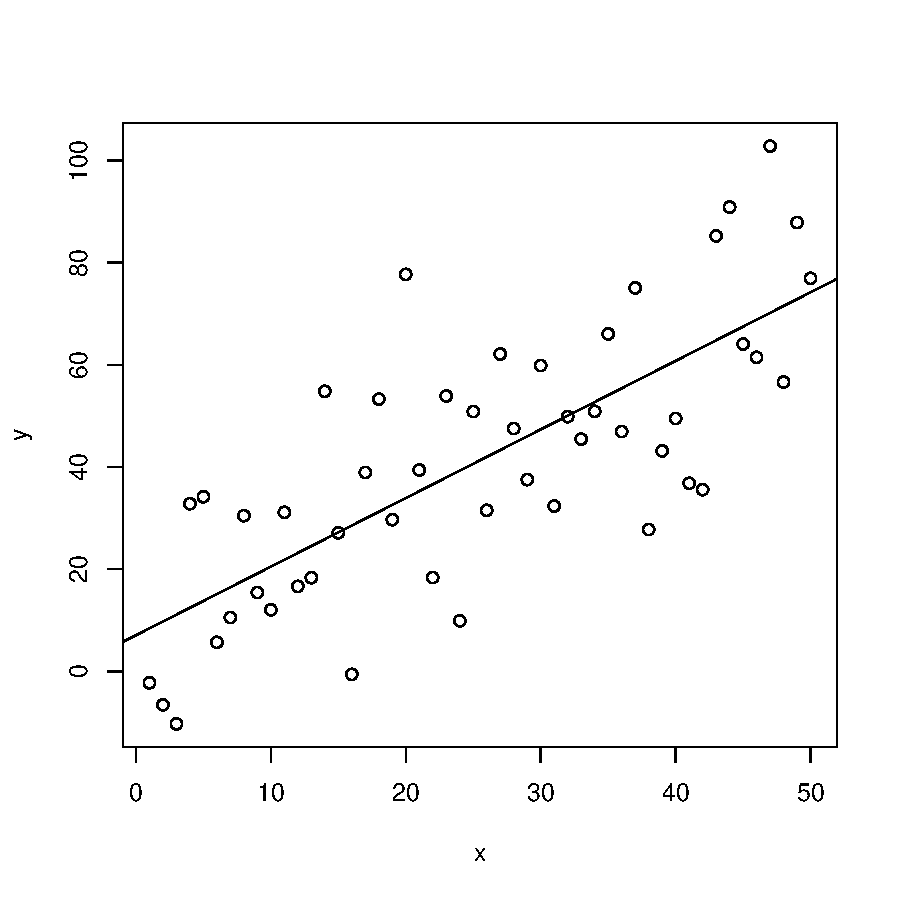
\includegraphics{plot_test-fig1}

\caption{Scatter Plot with Regression Line}
\label{fig:one}
\end{figure}
Note that \verb@x@, \verb@y@, and \verb@out1@ are remembered from
the preceding code chunk.  We don't have to regenerate them.
All code chunks are part of one R ``session''.


\end{document}
